\subsection*{What is a Plasma?}
    \noindent\makebox[\linewidth]{\rule{\textwidth}{0.4pt}}
    \begin{definition}[Plasma]
        ``Plasma'' refers here to an electrically charged fluid, typically occurring when a fluid is supplied with sufficient energy—from heating or an applied electromagnetic (EM) field—that a significant portion of the atoms \BA{(Not molecules?)} are ionised \BA{(Terminology?)}, causing the (positive) ion and (negative) electron phases to move independently.
    \end{definition}
    \noindent\makebox[\linewidth]{\rule{\textwidth}{0.4pt}}
    Plasma is one of the most abundant forms of matter in the universe \cite{CL13}, found most frequently in stars \cite{Phi95, Asc06, Pie17} and similarly—as in our case—the star-like environments emulated in a tokamak.
    
    While an applied EM field induces a current as it separates the two charged phases: the ions and electrons, the current similarly induces and EM field through Maxwell's equations, creating a complex, coupled, nonlinear system, referred to as magnetohydrodynamics (MHD). (See Figure \ref{fig:MHD coupling}) \BA{[Ref.]} This coupling is referred to as \emph{magnetohydrodynamics}, and is part of what makes the modelling and numerical simulation of plasma so complex and interesting.
    \begin{figure}[!h]
        \centering
        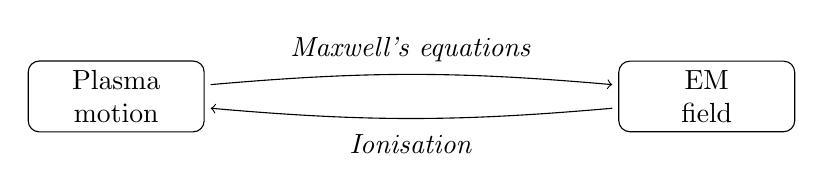
\begin{tikzpicture}[align = center, node distance = 4cm, auto]
            \node[draw = black, text width = 2cm, rounded corners] (1) at (0, 0) {Plasma \\ motion};
            \node[draw = black, text width = 2cm, rounded corners] (2) at (7.5, 0) {EM \\ field};
            
            \draw[->] (1.2, 0.15) to [out = 5, in = 175] (6.3, 0.15);
            \node[] at (3.75, 0.6) {\emph{Maxwell's equations}};
            \draw[->] (6.3, -0.15) to [out = 185, in = -5] (1.2, -0.15);
            \node[] at (3.75, -0.6) {\emph{Ionisation}};
        \end{tikzpicture}
        \caption{Coupling of the plasma motion and EM field in MHD.}
        \label{fig:MHD coupling}
    \end{figure}
    